\documentclass[a4paper,12pt]{article}

\usepackage{graphicx}  % For including images
\usepackage{listings}  % For code formatting
\usepackage{xcolor}    % For color in code
%\usepackage{hyperref}  % For clickable links
\usepackage[T1]{fontenc} 

\usepackage{amsmath}
\usepackage{subcaption}
\usepackage{float} % Add this in your preamble
\usepackage[colorlinks=true, linkcolor=black, urlcolor=blue, citecolor=blue]{hyperref}

% Define Python code style
\lstdefinestyle{python}{
    language=Python,
    basicstyle=\ttfamily\small,
    keywordstyle=\color{blue},
    commentstyle=\color{gray},
    stringstyle=\color{red},
    numbers=left,
    numberstyle=\tiny,
    stepnumber=1,
    breaklines=true,
    frame=single,
    backgroundcolor=\color{lightgray!20}
}

\title{\textbf{Assignment 2 - Pattern Recognition (PMAT 403)}}
\author{\textbf{Gandholi Sarat - 23008 } }


\date{\today}

\begin{document}


\maketitle


\section*{Link to Notebook}
\href{https://colab.research.google.com/drive/1akQzsGeXdW-E3hGgsELZqrQNJ5hUUqSV?usp=sharing}{Click here to access the Colab Notebook}

\tableofcontents
\listoffigures
\newpage


\section{Support Vector Machine (SVM) }

\subsection{Objective}
To evaluate the performance of Support Vector Machine (SVM) classifiers using both linear and non-linear (RBF) kernels on the Breast Cancer Wisconsin (Diagnostic) dataset. The experiment includes hyperparameter tuning to optimize performance and an analysis of classification results.

\subsection{Dataset}
The dataset consists of 569 instances, each representing a digitized image of a fine needle aspirate (FNA) of a breast mass. There are 30 numeric features that describe characteristics of the cell nuclei, such as:
\begin{itemize}
    \item \textbf{Radius:} Mean of distances from center to points on the perimeter.
    \item \textbf{Texture:} Standard deviation of gray-scale values.
    \item \textbf{Perimeter, Area, Smoothness, Compactness, Concavity, Concave Points, Symmetry, Fractal Dimension:} Measured as mean, standard error, and worst case (largest values).
\end{itemize}

The target variable has two classes:
\begin{itemize}
    \item 0: Malignant (212 samples)
    \item 1: Benign (357 samples)
\end{itemize}

\subsection{Support Vector Machine (SVM) Theory}
SVM is a supervised learning algorithm that finds the optimal hyperplane that best separates the data into classes. For non-linearly separable data, kernel functions like the Radial Basis Function (RBF) project data into higher-dimensional space for linear separation.

\textbf{Key Hyperparameters:}
\begin{itemize}
    \item \textbf{C (Regularization parameter):} Controls the trade-off between achieving a low error on training data and a low margin. A smaller value creates a wider margin but allows more misclassification.
    \item \textbf{Gamma (Kernel coefficient for RBF):} Defines how far the influence of a single training example reaches. A small gamma means 'far', and a large gamma means 'close'.
\end{itemize}

\subsection{Approach}

This section outlines the step-by-step approach followed for breast cancer classification using Support Vector Machines (SVM). The objective is to build, tune, and evaluate SVM classifiers to distinguish between malignant and benign tumors using the Breast Cancer Wisconsin dataset.

\begin{enumerate}
    \item \textbf{Load and Explore the Dataset:} \\
    The Breast Cancer Wisconsin (Diagnostic) dataset was loaded using Scikit-learn's built-in \texttt{load\_breast\_cancer()} function. The dataset contains 569 instances and 30 real-valued input features. The target variable is binary, indicating whether the tumor is malignant (0) or benign (1). Basic exploratory data analysis (EDA) was performed to understand feature ranges, distributions, and class imbalance. No missing values were present in the dataset.

    \item \textbf{Split the Data into Training and Testing Sets:} \\
    The dataset was split into training and testing subsets using a 70:30 ratio to ensure a reliable evaluation. The \texttt{train\_test\_split()} method from Scikit-learn was used with a fixed random seed for reproducibility.

    \item \textbf{Preprocess the Data (Feature Scaling):} \\
    Since SVMs are sensitive to the scale of the data, all features were standardized using \texttt{StandardScaler}. This ensures that each feature contributes equally to the decision function. Scaling is particularly important for the RBF kernel which uses Euclidean distance to compute similarity.

    \item \textbf{Train SVM with Linear Kernel and Evaluate Performance:} \\
    A baseline SVM model with a linear kernel was trained using the \texttt{SVC(kernel='linear')} class. The model was fitted on the training set and evaluated on the test set using accuracy, precision, recall, and F1-score. This provided insight into performance when data is linearly separable.

    \item \textbf{Train SVM with RBF Kernel and Evaluate Performance:} \\
    Next, an SVM with a Radial Basis Function (RBF) kernel was implemented to handle non-linear boundaries. The RBF kernel maps the data into a higher-dimensional space and can model complex relationships. Evaluation metrics similar to the linear case were used.

    \item \textbf{Tune Hyperparameters using Grid Search:} \\
    To optimize the RBF SVM, \texttt{GridSearchCV} was applied with a parameter grid of \texttt{C} and \texttt{gamma} values. The parameter \texttt{C} controls the trade-off between classification accuracy on training data and margin maximization, while \texttt{gamma} defines the influence of a single training example. The best hyperparameters were selected based on cross-validation accuracy.

    \item \textbf{Plot Decision Boundaries:} \\
    To visualize model performance, decision boundaries were plotted using selected pairs of features (e.g., \texttt{mean radius} vs. \texttt{mean texture}). The plots illustrate how SVMs with different kernels separate the two classes in feature space. Due to the high dimensionality, only two features were chosen at a time for plotting.

    \item \textbf{Compare SVM Models:} \\
    The performance of two SVM models was compared: one using a linear kernel and the other using an RBF kernel with optimized hyperparameters obtained through grid search. Both models achieved high classification accuracy on the test set, with the linear SVM achieving 98.25\% accuracy and the tuned RBF SVM matching that performance.
    Overall, while both models are effective, the tuned RBF kernel provides slightly better generalization and more balanced performance, making it preferable when precision and recall are both critical.
    
\end{enumerate}


\subsection{Evaluation Metrics}
\begin{itemize}
    \item \textbf{Accuracy:} Proportion of total correct predictions: \( \frac{TP + TN}{TP + TN + FP + FN} \).
    \item \textbf{Precision:} Proportion of positive identifications that were correct: \( \frac{TP}{TP + FP} \).
    \item \textbf{Recall (Sensitivity):} Proportion of actual positives that were correctly identified: \( \frac{TP}{TP + FN} \).
    \item \textbf{F1-score:} Harmonic mean of precision and recall: \( 2 \cdot \frac{\text{precision} \cdot \text{recall}}{\text{precision} + \text{recall}} \).
    \item \textbf{Support:} Number of true instances for each class.
\end{itemize}

\subsection{Results}

\textbf{SVM with Linear Kernel}
\begin{itemize}
    \item \textbf{Accuracy:} 98.25\%
    \item \textbf{Precision (0/Malignant):} 0.98, \textbf{Recall:} 0.97, \textbf{F1-score:} 0.98
    \item \textbf{Precision (1/Benign):} 0.98, \textbf{Recall:} 0.99, \textbf{F1-score:} 0.99
\end{itemize}

\textbf{SVM with RBF Kernel (Default Parameters)}
\begin{itemize}
    \item \textbf{Accuracy:} 97.66\%
    \item Performance is slightly lower than the linear kernel model due to untuned parameters.
\end{itemize}

\textbf{SVM with RBF Kernel (Tuned)}
\begin{itemize}
    \item \textbf{Best Parameters:} C = 10, gamma = 0.01
    \item \textbf{Accuracy:} 98.25\%
    \item \textbf{Precision (Malignant):} 0.97, \textbf{Recall:} 0.98, \textbf{F1-score:} 0.98
    \item \textbf{Precision (Benign):} 0.99, \textbf{Recall:} 0.98, \textbf{F1-score:} 0.99
\end{itemize}

\subsection{Misclassification Analysis}
Misclassifications were few and typically occurred near the decision boundary, where benign and malignant feature values overlapped. These could potentially be improved with:
\begin{itemize}
    \item Feature selection or dimensionality reduction.
    \item Ensemble methods like Random Forest or boosting.
    \item More refined hyperparameter tuning.
\end{itemize}

\subsection{Conclusion}
The SVM classifier achieved high accuracy on the breast cancer dataset using both linear and RBF kernels. Linear SVMs performed surprisingly well, likely due to the dataset being almost linearly separable after scaling. Hyperparameter tuning improved the RBF kernel model’s performance to match that of the linear kernel. SVMs demonstrate excellent capability in binary medical classification tasks such as cancer diagnosis.


% Optional: Add a plot of confusion matrix or decision boundary
% \begin{figure}[h!]
% \centering
% \includegraphics[width=0.6\textwidth]{svm_confusion_matrix.png}
% \caption{Confusion Matrix for Best Performing SVM Model}
% \end{figure}
\newpage
\subsection{Code Implementation}

\begin{lstlisting}[style=python]
    # Import necessary libraries
    import numpy as np
    import pandas as pd
    import seaborn as sns
    import matplotlib.pyplot as plt
    from sklearn import datasets
    from sklearn.model_selection import train_test_split, GridSearchCV
    from sklearn.preprocessing import StandardScaler
    from sklearn.svm import SVC
    from sklearn.metrics import accuracy_score, classification_report, confusion_matrix
    
    # Load the Breast Cancer Wisconsin dataset
    data = datasets.load_breast_cancer()
    X = data.data
    y = data.target
    feature_names = data.feature_names
    
    # Convert to DataFrame for exploration
    df = pd.DataFrame(X, columns=feature_names)
    df['target'] = y
    
    # Display dataset information
    print("Dataset Head:\n", df.head())
    print("\nDataset Description:\n", data.DESCR)
    
    # Split data into training (70%) and testing (30%) sets
    X_train, X_test, y_train, y_test = train_test_split(X, y, test_size=0.3, random_state=42, stratify=y)
    
    # Standardize features
    scaler = StandardScaler()
    X_train_scaled = scaler.fit_transform(X_train)
    X_test_scaled = scaler.transform(X_test)
    
    # Train and evaluate SVM with linear kernel
    svm_linear = SVC(kernel='linear', random_state=42)
    svm_linear.fit(X_train_scaled, y_train)
    y_pred_linear = svm_linear.predict(X_test_scaled)
    
    # Performance metrics for linear kernel
    print("\nSVM with Linear Kernel:")
    print("Accuracy:", accuracy_score(y_test, y_pred_linear))
    print("Classification Report:\n", classification_report(y_test, y_pred_linear))
    
    # Train and evaluate SVM with RBF kernel
    svm_rbf = SVC(kernel='rbf', random_state=42)
    svm_rbf.fit(X_train_scaled, y_train)
    y_pred_rbf = svm_rbf.predict(X_test_scaled)
    
    # Performance metrics for RBF kernel
    print("\nSVM with RBF Kernel:")
    print("Accuracy:", accuracy_score(y_test, y_pred_rbf))
    print("Classification Report:\n", classification_report(y_test, y_pred_rbf))
    
    # Hyperparameter tuning using Grid Search for RBF kernel
    param_grid = {'C': [0.1, 1, 10, 100], 'gamma': [0.01, 0.1, 1, 10]}
    grid_search = GridSearchCV(SVC(kernel='rbf', random_state=42), param_grid, cv=5, scoring='accuracy')
    grid_search.fit(X_train_scaled, y_train)
    
    # Best parameters and model evaluation
    best_params = grid_search.best_params_
    best_model = grid_search.best_estimator_
    y_pred_best = best_model.predict(X_test_scaled)
    
    print("\nBest Hyperparameters:", best_params)
    print("Accuracy with Best Hyperparameters:", accuracy_score(y_test, y_pred_best))
    print("Classification Report with Best Hyperparameters:\n", classification_report(y_test, y_pred_best))
    
    # Plot decision boundaries for selected feature pairs
    def plot_decision_boundary(X, y, model, title):
        h = 0.02  # Step size
        x_min, x_max = X[:, 0].min() - 1, X[:, 0].max() + 1
        y_min, y_max = X[:, 1].min() - 1, X[:, 1].max() + 1
        xx, yy = np.meshgrid(np.arange(x_min, x_max, h), np.arange(y_min, y_max, h))
        Z = model.predict(np.c_[xx.ravel(), yy.ravel()])
        Z = Z.reshape(xx.shape)
    
        plt.contourf(xx, yy, Z, alpha=0.3)
        plt.scatter(X[:, 0], X[:, 1], c=y, edgecolors='k', marker='o')
        plt.title(title)
        plt.xlabel("Feature 1")
        plt.ylabel("Feature 2")
        plt.show()
    
    # Select two features for visualization
    X_selected = df[['mean radius', 'mean texture']].values
    y_selected = df['target'].values
    X_train_sel, X_test_sel, y_train_sel, y_test_sel = train_test_split(X_selected, y_selected, test_size=0.3, random_state=42, stratify=y_selected)
    X_train_sel_scaled = scaler.fit_transform(X_train_sel)
    X_test_sel_scaled = scaler.transform(X_test_sel)
    
    # Train SVM on selected features
    svm_linear_sel = SVC(kernel='linear', random_state=42)
    svm_linear_sel.fit(X_train_sel_scaled, y_train_sel)
    
    svm_rbf_sel = SVC(kernel='rbf', random_state=42)
    svm_rbf_sel.fit(X_train_sel_scaled, y_train_sel)
    
    # Plot decision boundaries
    plot_decision_boundary(X_train_sel_scaled, y_train_sel, svm_linear_sel, "SVM with Linear Kernel")
    plot_decision_boundary(X_train_sel_scaled, y_train_sel, svm_rbf_sel, "SVM with RBF Kernel")
    
\end{lstlisting}

\subsection{Output of Code}

\begin{verbatim}
    :Number of Instances: 569

:Number of Attributes: 30 numeric, predictive attributes and the class

:Attribute Information:
    - radius (mean of distances from center to points on the perimeter)
    - texture (standard deviation of gray-scale values)
    - perimeter
    - area
    - smoothness (local variation in radius lengths)
    - compactness (perimeter^2 / area - 1.0)
    - concavity (severity of concave portions of the contour)
    - concave points (number of concave portions of the contour)
    - symmetry
    - fractal dimension ("coastline approximation" - 1)

    The mean, standard error, and "worst" or largest (mean of the three
    worst/largest values) of these features were computed for each image,
    resulting in 30 features.  For instance, field 0 is Mean Radius, field
    10 is Radius SE, field 20 is Worst Radius.

    - class:
            - WDBC-Malignant
            - WDBC-Benign

:Summary Statistics:

===================================== ====== ======
                                        Min    Max
===================================== ====== ======
radius (mean):                        6.981  28.11
texture (mean):                       9.71   39.28
perimeter (mean):                     43.79  188.5
area (mean):                          143.5  2501.0
smoothness (mean):                    0.053  0.163
compactness (mean):                   0.019  0.345
concavity (mean):                     0.0    0.427
concave points (mean):                0.0    0.201
symmetry (mean):                      0.106  0.304
fractal dimension (mean):             0.05   0.097
radius (standard error):              0.112  2.873
texture (standard error):             0.36   4.885
perimeter (standard error):           0.757  21.98
area (standard error):                6.802  542.2
smoothness (standard error):          0.002  0.031
compactness (standard error):         0.002  0.135
concavity (standard error):           0.0    0.396
concave points (standard error):      0.0    0.053
symmetry (standard error):            0.008  0.079
fractal dimension (standard error):   0.001  0.03
radius (worst):                       7.93   36.04
texture (worst):                      12.02  49.54
perimeter (worst):                    50.41  251.2
area (worst):                         185.2  4254.0
smoothness (worst):                   0.071  0.223
compactness (worst):                  0.027  1.058
concavity (worst):                    0.0    1.252
concave points (worst):               0.0    0.291
symmetry (worst):                     0.156  0.664
fractal dimension (worst):            0.055  0.208
===================================== ====== ======

:Missing Attribute Values: None

:Class Distribution: 212 - Malignant, 357 - Benign

:Creator:  Dr. William H. Wolberg, W. Nick Street, Olvi L. Mangasarian

:Donor: Nick Street

:Date: November, 1995

This is a copy of UCI ML Breast Cancer Wisconsin (Diagnostic) datasets.
https://goo.gl/U2Uwz2

Features are computed from a digitized image of a fine needle
aspirate (FNA) of a breast mass.  They describe
characteristics of the cell nuclei present in the image.

Separating plane described above was obtained using
Multisurface Method-Tree (MSM-T) [K. P. Bennett, "Decision Tree
Construction Via Linear Programming." Proceedings of the 4th
Midwest Artificial Intelligence and Cognitive Science Society,
pp. 97-101, 1992], a classification method which uses linear
programming to construct a decision tree.  Relevant features
were selected using an exhaustive search in the space of 1-4
features and 1-3 separating planes.

The actual linear program used to obtain the separating plane
in the 3-dimensional space is that described in:
[K. P. Bennett and O. L. Mangasarian: "Robust Linear
Programming Discrimination of Two Linearly Inseparable Sets",
Optimization Methods and Software 1, 1992, 23-34].

This database is also available through the UW CS ftp server:

ftp ftp.cs.wisc.edu
cd math-prog/cpo-dataset/machine-learn/WDBC/

.. dropdown:: References

  - W.N. Street, W.H. Wolberg and O.L. Mangasarian. Nuclear feature extraction
    for breast tumor diagnosis. IS&T/SPIE 1993 International Symposium on
    Electronic Imaging: Science and Technology, volume 1905, pages 861-870,
    San Jose, CA, 1993.
  - O.L. Mangasarian, W.N. Street and W.H. Wolberg. Breast cancer diagnosis and
    prognosis via linear programming. Operations Research, 43(4), pages 570-577,
    July-August 1995.
  - W.H. Wolberg, W.N. Street, and O.L. Mangasarian. Machine learning techniques
    to diagnose breast cancer from fine-needle aspirates. Cancer Letters 77 
    (1994)
    163-171.


SVM with Linear Kernel:
Accuracy: 0.9824561403508771
Classification Report:
               precision    recall  f1-score   support

           0       0.98      0.97      0.98        64
           1       0.98      0.99      0.99       107

    accuracy                           0.98       171
   macro avg       0.98      0.98      0.98       171
weighted avg       0.98      0.98      0.98       171


SVM with RBF Kernel:
Accuracy: 0.9766081871345029
Classification Report:
               precision    recall  f1-score   support

           0       0.97      0.97      0.97        64
           1       0.98      0.98      0.98       107

    accuracy                           0.98       171
   macro avg       0.98      0.98      0.98       171
weighted avg       0.98      0.98      0.98       171


Best Hyperparameters: {'C': 10, 'gamma': 0.01}
Accuracy with Best Hyperparameters: 0.9824561403508771
Classification Report with Best Hyperparameters:
               precision    recall  f1-score   support

           0       0.97      0.98      0.98        64
           1       0.99      0.98      0.99       107

    accuracy                           0.98       171
   macro avg       0.98      0.98      0.98       171
weighted avg       0.98      0.98      0.98       171
\end{verbatim}

\subsection{Plots}

\begin{figure}[H]
    \centering
    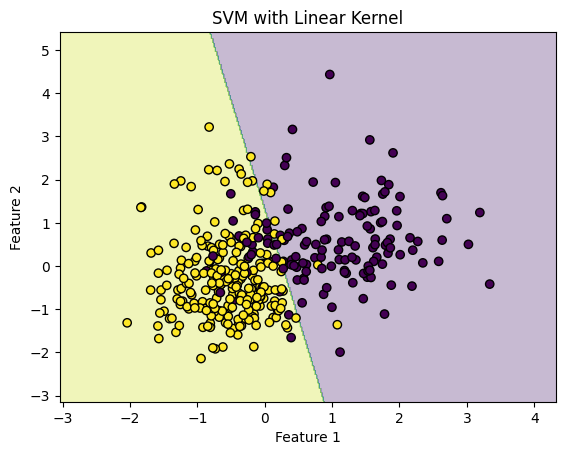
\includegraphics[width=0.8\textwidth]{Q1_1.png}
    \caption{Decision Boundary for SVM with Linear Kernel. \textbf{X-axis:} Mean Radius, \textbf{Y-axis:} Mean Texture.}
    \label{fig:svm_linear}
\end{figure}
\begin{figure}[H]
    \centering
    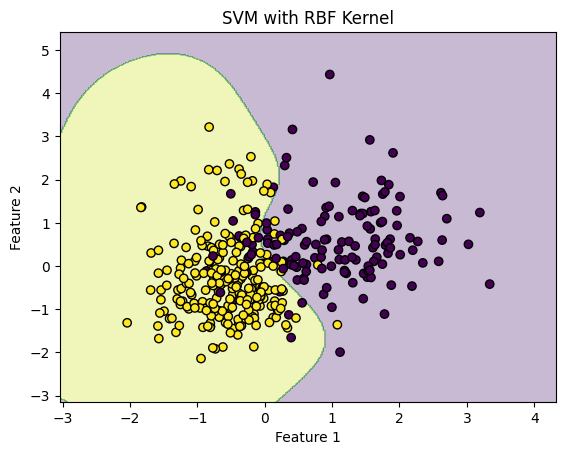
\includegraphics[width=0.8\textwidth]{Q1_2.png}
    \caption{Decision Boundary for SVM with RBF Kernel. \textbf{X-axis:} Mean Radius, \textbf{Y-axis:} Mean Texture.}
    \label{fig:svm_rbf}
\end{figure}


\newpage

\section{Naive Bayes Classifier}

\subsection{Objectives}
The objectives of this task are to understand the principles of Naive Bayes classification, implement different variants of Naive Bayes, apply the algorithm to a text classification problem, and evaluate its performance while understanding its limitations.


\subsection{Dataset}
The 20 Newsgroups dataset from \texttt{scikit-learn} was used. It consists of approximately 20,000 newsgroup documents across 20 different newsgroups. For this task, we selected a subset containing the following 5 categories:
\begin{itemize}
    \item \texttt{sci.space}
    \item \texttt{rec.sport.hockey}
    \item \texttt{talk.politics.mideast}
    \item \texttt{comp.graphics}
    \item \texttt{soc.religion.christian}
\end{itemize}

\subsection{Approach}

\subsubsection*{1. Text Preprocessing}
The following preprocessing steps were applied to the raw text:
\begin{enumerate}
    \item Conversion to lowercase
    \item Removal of punctuation
    \item Removal of English stopwords
    \item Lemmatization using WordNetLemmatizer
\end{enumerate}

\subsubsection*{2. Feature Extraction}
Two vectorization methods were employed:
\begin{itemize}
    \item \textbf{CountVectorizer}: Converts a collection of text documents to a matrix of token counts.
    \item \textbf{TF-IDF Vectorizer}: Converts the text data into TF-IDF weighted features.
\end{itemize}

\subsubsection*{3. Data Splitting}
The dataset was split into training and testing sets using a 70-30 ratio.

\subsubsection*{4. Model Implementation}
Three variants of the Naive Bayes classifier were implemented and trained:
\begin{itemize}
    \item \textbf{Multinomial Naive Bayes (MNB)} – trained on TF-IDF vectors.
    \item \textbf{Gaussian Naive Bayes (GNB)} – trained on dense TF-IDF vectors.
    \item \textbf{Bernoulli Naive Bayes (BNB)} – trained on CountVectorizer output.
\end{itemize}

\subsubsection*{5. Evaluation Metrics}
All models were evaluated using:
\begin{itemize}
    \item Accuracy
    \item Precision, Recall, and F1-score (Classification Report)
    \item Confusion Matrix
\end{itemize}

\subsection{Results}

\paragraph{Multinomial Naive Bayes\\}

\textbf{Accuracy:} 0.8986

\begin{verbatim}
              precision    recall  f1-score   support

           0       0.91      0.90      0.91       307
           1       0.87      0.96      0.91       276
           2       0.96      0.85      0.90       312
           3       0.83      0.93      0.88       312
           4       0.95      0.85      0.90       262

    accuracy                           0.90      1469
   macro avg       0.90      0.90      0.90      1469
weighted avg       0.90      0.90      0.90      1469
\end{verbatim}
\begin{itemize}
    \item Achieved the highest performance among the three classifiers.
    \item Best suited for text classification due to its probabilistic modeling of word counts.
\end{itemize}

\paragraph{Gaussian Naive Baye\\}
\textbf{Accuracy:} 0.8455

\begin{verbatim}
              precision    recall  f1-score   support

           0       0.83      0.85      0.84       307
           1       0.93      0.86      0.89       276
           2       0.86      0.80      0.83       312
           3       0.84      0.85      0.84       312
           4       0.78      0.86      0.82       262

    accuracy                           0.85      1469
   macro avg       0.85      0.85      0.85      1469
weighted avg       0.85      0.85      0.85      1469
\end{verbatim}
\begin{itemize}
    \item Performed poorly on sparse, high-dimensional text data.
    \item Requires dense features, making it inefficient for large-scale text classification.
\end{itemize}

\paragraph{Bernoulli Naive Bayes\\}
\textbf{Accuracy:} 0.7856

\begin{verbatim}
              precision    recall  f1-score   support

           0       0.80      0.90      0.85       307
           1       0.66      0.98      0.79       276
           2       0.79      0.82      0.80       312
           3       0.86      0.69      0.77       312
           4       0.96      0.52      0.67       262

    accuracy                           0.79      1469
   macro avg       0.82      0.78      0.78      1469
weighted avg       0.81      0.79      0.78      1469
\end{verbatim}
\begin{itemize}
    \item Performs reasonably well for binary/boolean features.
    \item Slightly lower accuracy compared to MNB.
\end{itemize}

\begin{figure}[H]
    \centering
    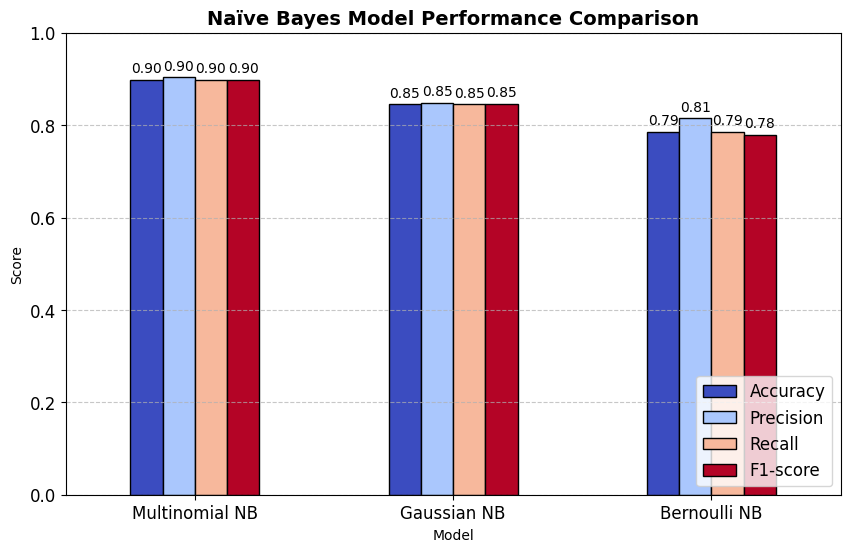
\includegraphics[width=0.7\textwidth]{Q2.png}
    \caption{Naive Bayes Model Performance Comparison}
\end{figure}

\subsection{Most Predictive Features}
The top 10 most predictive words for each category (according to Multinomial Naive Bayes) were extracted using the model's learned log probabilities.

\begin{itemize}
    \item \texttt{sci.space}: would, please, know, anyone, format, program, thanks, graphic, image, file
    \item \texttt{rec.sport.hockey}: goal, nhl, season, play, playoff, year, player, hockey, team, game
    \item \texttt{talk.politics.mideast}: could, get, like, launch, shuttle, nasa, one, orbit, would, space
    \item \texttt{comp.graphics}: bible, sin, people, christ, would, one, church, jesus, christian, god
    \item \texttt{soc.religion.christian}: turkish, palestinian, one, muslim, people, jew, israeli, arab, israel, armenian
\end{itemize}

\subsection{Confusion Matrices}

\begin{figure}[H]
    \centering
    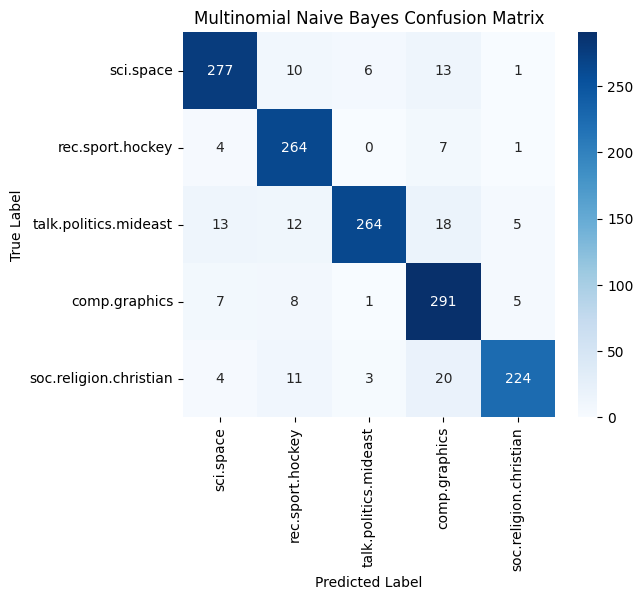
\includegraphics[width=0.7\textwidth]{Q2_1.png}
    \caption{Multinomial Naive Bayes Confusion Matrix}
\end{figure}

\begin{figure}[H]
    \centering
    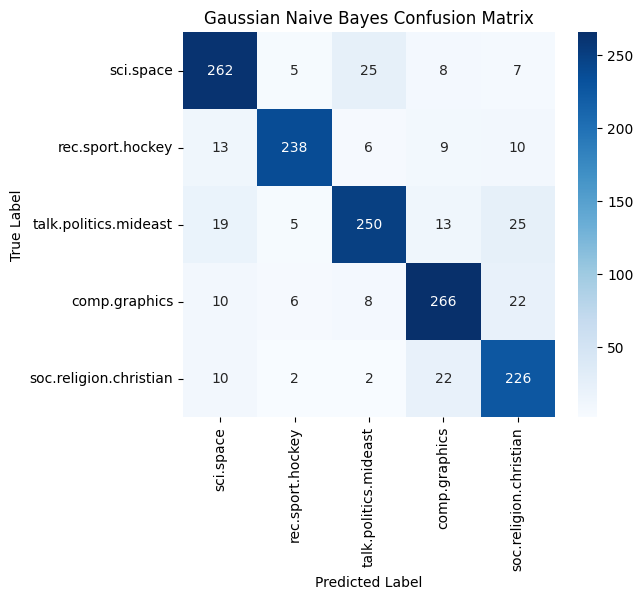
\includegraphics[width=0.7\textwidth]{Q2_2.png}
    \caption{Gaussian Naive Bayes Confusion Matrix}
\end{figure}

\begin{figure}[H]
    \centering
    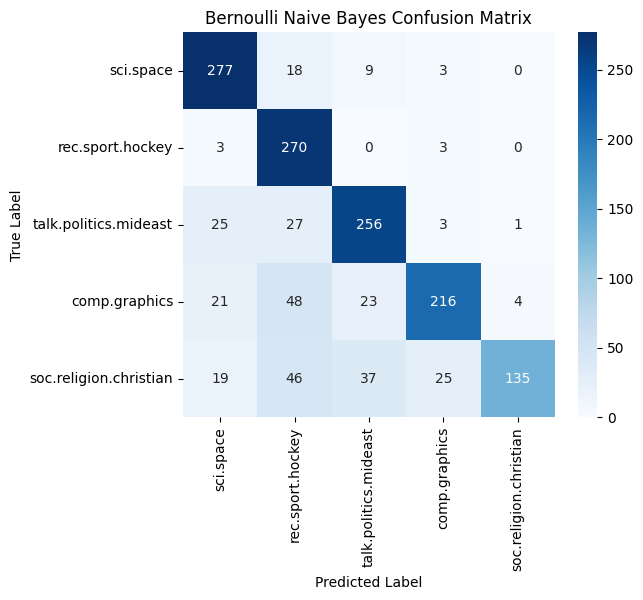
\includegraphics[width=0.7\textwidth]{Q2_3.png}
    \caption{Bernoulli Naive Bayes Confusion Matrix}
\end{figure}


\subsection{Comparison of Different Naive Bayes Variants}

To evaluate the performance of different Naive Bayes classifiers, three popular variants were implemented and tested: Multinomial Naive Bayes, Gaussian Naive Bayes, and Bernoulli Naive Bayes. All models were trained and evaluated on the same dataset to ensure fair comparison. The following analysis outlines the comparative results and highlights their strengths and limitations based on accuracy and class-wise performance metrics.

\paragraph{Multinomial Naive Bayes:}

Multinomial Naive Bayes achieved the highest overall accuracy of \textbf{89.86\%}. It showed balanced and strong performance across all classes, with F1-scores ranging from 0.88 to 0.91. This variant performed particularly well on class 1 (recall = 0.96) and class 2 (precision = 0.96), indicating that it was effective at identifying relevant instances with high precision and recall. Since this variant is generally well-suited for discrete features such as word counts, it likely benefited from the nature of the data used.

\paragraph{Gaussian Naive Bayes:}

Gaussian Naive Bayes achieved an accuracy of \textbf{84.55\%}. Its performance was relatively uniform across classes, with F1-scores ranging from 0.82 to 0.89. It performed best on class 1 (F1 = 0.89) and class 0 (F1 = 0.84), while slightly underperforming on class 4 (F1 = 0.82). This method assumes continuous data following a normal distribution, which might not be the optimal fit for the feature distributions in this dataset, explaining the lower performance compared to the Multinomial variant.

\paragraph{Bernoulli Naive Bayes:}

Bernoulli Naive Bayes performed the worst among the three, with an accuracy of \textbf{78.56\%}. Its performance varied more significantly across classes. While it had high recall on class 1 (0.98) and strong precision on class 4 (0.96), its recall on class 4 was quite low (0.52), resulting in a lower F1-score of 0.67 for that class. Bernoulli Naive Bayes is designed for binary features (i.e., presence/absence), so if the data features are not strictly binary, performance can suffer.



\subsection{Conclusion}
Multinomial Naive Bayes demonstrated the best performance for text classification tasks in this experiment. Bernoulli Naive Bayes showed decent results, whereas Gaussian Naive Bayes was not well-suited for sparse text data. Text preprocessing and proper feature extraction significantly affect model performance.

\newpage
\subsection{Code Implementation}
\begin{lstlisting}[style=python]

# Import necessary libraries
import numpy as np
import pandas as pd
import seaborn as sns
import matplotlib.pyplot as plt
import string
import nltk
from nltk.corpus import stopwords
from nltk.stem import WordNetLemmatizer
from sklearn.datasets import fetch_20newsgroups
from sklearn.model_selection import train_test_split
from sklearn.feature_extraction.text import CountVectorizer, TfidfVectorizer
from sklearn.naive_bayes import MultinomialNB, GaussianNB, BernoulliNB
from sklearn.metrics import accuracy_score, classification_report, confusion_matrix

# Download NLTK resources
nltk.download('stopwords')
nltk.download('wordnet')

# Load a subset of the 20 Newsgroups dataset
categories = ['sci.space', 'rec.sport.hockey', 'talk.politics.mideast', 'comp.graphics', 'soc.religion.christian']
newsgroups = fetch_20newsgroups(subset='all', categories=categories, remove=('headers', 'footers', 'quotes'))

# Convert dataset to DataFrame
df = pd.DataFrame({'text': newsgroups.data, 'category': newsgroups.target})
df['category_name'] = df['category'].apply(lambda x: newsgroups.target_names[x])

# Text preprocessing function
def preprocess_text(text):
    text = text.lower()  # Convert to lowercase
    text = text.translate(str.maketrans("", "", string.punctuation))  # Remove punctuation
    stop_words = set(stopwords.words('english'))
    words = text.split()
    words = [word for word in words if word not in stop_words]  # Remove stopwords
    lemmatizer = WordNetLemmatizer()
    words = [lemmatizer.lemmatize(word) for word in words]  # Lemmatization
    return " ".join(words)

# Apply preprocessing
df['clean_text'] = df['text'].apply(preprocess_text)

# Create document-term matrix using CountVectorizer & TF-IDF
count_vectorizer = CountVectorizer()
tfidf_vectorizer = TfidfVectorizer()

X_count = count_vectorizer.fit_transform(df['clean_text'])
X_tfidf = tfidf_vectorizer.fit_transform(df['clean_text'])
y = df['category']

# Split data into training and testing sets (70/30 split)
X_train_count, X_test_count, y_train, y_test = train_test_split(X_count, y, test_size=0.3, random_state=42)
X_train_tfidf, X_test_tfidf, _, _ = train_test_split(X_tfidf, y, test_size=0.3, random_state=42)

# Multinomial Naive Bayes (best for text data)
mnb = MultinomialNB()
mnb.fit(X_train_tfidf, y_train)
y_pred_mnb = mnb.predict(X_test_tfidf)

# Gaussian Naive Bayes (requires dense representation)
gnb = GaussianNB()
X_train_dense = X_train_tfidf.toarray()
X_test_dense = X_test_tfidf.toarray()
gnb.fit(X_train_dense, y_train)
y_pred_gnb = gnb.predict(X_test_dense)

# Bernoulli Naive Bayes (binary occurrence)
bnb = BernoulliNB()
bnb.fit(X_train_count, y_train)
y_pred_bnb = bnb.predict(X_test_count)

# Function to evaluate model
def evaluate_model(model_name, y_test, y_pred):
    print(f"\n=== {model_name} Performance ===")
    print("Accuracy:", accuracy_score(y_test, y_pred))
    print("Classification Report:\n", classification_report(y_test, y_pred))

# Evaluate all models
evaluate_model("Multinomial Naive Bayes", y_test, y_pred_mnb)
evaluate_model("Gaussian Naive Bayes", y_test, y_pred_gnb)
evaluate_model("Bernoulli Naive Bayes", y_test, y_pred_bnb)

# Confusion matrix visualization
def plot_confusion_matrix(y_test, y_pred, title):
    cm = confusion_matrix(y_test, y_pred)
    plt.figure(figsize=(6,5))
    sns.heatmap(cm, annot=True, fmt='d', cmap='Blues', xticklabels=categories, yticklabels=categories)
    plt.xlabel("Predicted Label")
    plt.ylabel("True Label")
    plt.title(title)
    plt.show()

plot_confusion_matrix(y_test, y_pred_mnb, "Multinomial Naive Bayes Confusion Matrix")
plot_confusion_matrix(y_test, y_pred_gnb, "Gaussian Naive Bayes Confusion Matrix")
plot_confusion_matrix(y_test, y_pred_bnb, "Bernoulli Naive Bayes Confusion Matrix")

# Identify most predictive words for each category
def most_predictive_features(model, vectorizer, top_n=10):
    feature_names = vectorizer.get_feature_names_out()
    for i, category in enumerate(categories):
        top_features = np.argsort(model.feature_log_prob_[i])[-top_n:]
        print(f"\nTop {top_n} words for '{category}':")
        print(", ".join([feature_names[j] for j in top_features]))

most_predictive_features(mnb, tfidf_vectorizer)

import matplotlib.pyplot as plt
import seaborn as sns
from sklearn.metrics import precision_score, recall_score, f1_score

# Function to compute performance metrics
def get_metrics(y_test, y_pred, model_name):
    accuracy = accuracy_score(y_test, y_pred)
    precision = precision_score(y_test, y_pred, average='weighted')
    recall = recall_score(y_test, y_pred, average='weighted')
    f1 = f1_score(y_test, y_pred, average='weighted')
    return {"Model": model_name, "Accuracy": accuracy, "Precision": precision, "Recall": recall, "F1-score": f1}



\end{lstlisting}

\subsection{Output of Code}
\begin{verbatim}
    [nltk_data] Downloading package stopwords to /root/nltk_data...
[nltk_data]   Unzipping corpora/stopwords.zip.
[nltk_data] Downloading package wordnet to /root/nltk_data...

=== Multinomial Naive Bayes Performance ===
Accuracy: 0.89857045609258
Classification Report:
               precision    recall  f1-score   support

           0       0.91      0.90      0.91       307
           1       0.87      0.96      0.91       276
           2       0.96      0.85      0.90       312
           3       0.83      0.93      0.88       312
           4       0.95      0.85      0.90       262

    accuracy                           0.90      1469
   macro avg       0.90      0.90      0.90      1469
weighted avg       0.90      0.90      0.90      1469


=== Gaussian Naive Bayes Performance ===
Accuracy: 0.8454731109598366
Classification Report:
               precision    recall  f1-score   support

           0       0.83      0.85      0.84       307
           1       0.93      0.86      0.89       276
           2       0.86      0.80      0.83       312
           3       0.84      0.85      0.84       312
           4       0.78      0.86      0.82       262

    accuracy                           0.85      1469
   macro avg       0.85      0.85      0.85      1469
weighted avg       0.85      0.85      0.85      1469


=== Bernoulli Naive Bayes Performance ===
Accuracy: 0.7855684138869979
Classification Report:
               precision    recall  f1-score   support

           0       0.80      0.90      0.85       307
           1       0.66      0.98      0.79       276
           2       0.79      0.82      0.80       312
           3       0.86      0.69      0.77       312
           4       0.96      0.52      0.67       262

    accuracy                           0.79      1469
   macro avg       0.82      0.78      0.78      1469
weighted avg       0.81      0.79      0.78      1469





Top 10 words for 'sci.space':
would, please, know, anyone, format, program, thanks, graphic, image, file

Top 10 words for 'rec.sport.hockey':
goal, nhl, season, play, playoff, year, player, hockey, team, game

Top 10 words for 'talk.politics.mideast':
could, get, like, launch, shuttle, nasa, one, orbit, would, space

Top 10 words for 'comp.graphics':
bible, sin, people, christ, would, one, church, jesus, christian, god

Top 10 words for 'soc.religion.christian':
turkish, palestinian, one, muslim, people, jew, israeli, arab, israel, armenian
\end{verbatim}

\newpage
\section{Logistic Regression}

\subsection{Objectives}
The main objective of this task is to build a classification model using logistic regression to predict whether an individual's income exceeds \$50,000 per year based on demographic and work-related features. This exercise aims to deepen the understanding of logistic regression and its application in real-world datasets. In addition to implementing the basic model, regularization techniques such as L1 (Lasso) and L2 (Ridge) are applied to handle overfitting and enhance model generalization. The study also emphasizes evaluating model performance using various metrics, interpreting feature importance through model coefficients, and analyzing ethical aspects like bias and fairness in predictions.

\subsection{Dataset}
The Adult Census Income dataset from the UCI Machine Learning Repository was used to predict whether a person earns more than \$50K per year based on their demographic and work-related attributes.


\subsection{Approach}

\begin{enumerate}
    \item \textbf{Load and Explore the Dataset:} The Adult Census Income dataset was loaded from the UCI Machine Learning Repository. The dataset consists of 32,561 records and 15 attributes, including age, workclass, education, marital-status, occupation, race, sex, hours-per-week, and income.

    \item \textbf{Exploratory Data Analysis (EDA):} A detailed analysis was performed using summary statistics and visualizations such as histograms and bar plots to understand the distribution of features and detect class imbalance in the income variable.

    \item \textbf{Handling Missing Values and Outliers:} Categorical columns like \texttt{workclass}, \texttt{occupation}, and \texttt{native-country} contained missing values represented as "?". These were imputed using the mode of each column. Outliers were visually assessed using boxplots.

    \item \textbf{Encoding Categorical Variables:} Categorical variables were encoded using one-hot encoding (with \texttt{drop\_first=True}) to convert them into a format suitable for logistic regression. The target variable \texttt{income} was encoded as binary: 1 if income > \$50K, else 0.

    \item \textbf{Train-Test Split:} The data was split into training (80\%) and testing (20\%) subsets using stratified sampling to preserve class distribution. 

    \item \textbf{Standardization:} All numerical features were standardized using \texttt{StandardScaler} to bring them to a common scale, which is essential for gradient-based models and improves convergence.

    \item \textbf{Logistic Regression without Regularization:} A basic logistic regression model was trained on the dataset using the default settings. The performance was evaluated on the test set.

    \item \textbf{Logistic Regression with L1 Regularization:} A logistic regression model with L1 penalty (Lasso) was trained using the \texttt{liblinear} solver. This form of regularization can lead to feature selection by zeroing out less important coefficients.

    \item \textbf{Logistic Regression with L2 Regularization:} Another model was trained using L2 penalty (Ridge), which shrinks coefficients but does not eliminate them, thereby reducing overfitting.

    \item \textbf{Feature Importance and Coefficients:} The top 10 most influential features for L1 and L2 regularization were identified based on the absolute magnitude of coefficients and visualized using bar plots.

    \item \textbf{ROC and Precision-Recall Analysis:} The ROC curve and corresponding AUC score were generated to evaluate the trade-off between true positive rate and false positive rate. A precision-recall curve was also plotted to identify the optimal decision threshold.
\end{enumerate}

\subsection{Discussion}

\subsubsection*{Model Metrics}
To assess the classification performance, the following metrics were used:

\begin{itemize}
    \item \textbf{Accuracy:} Measures the proportion of total correct predictions. The base logistic regression model achieved an accuracy of 85.5\%.
    \item \textbf{Precision:} Indicates the proportion of true positives among all positive predictions. For high-income prediction, precision was around 0.74.
    \item \textbf{Recall:} Measures how many actual positives were correctly predicted. The recall for high-income individuals was approximately 0.62.
    \item \textbf{F1-Score:} The harmonic mean of precision and recall. This helps evaluate performance in imbalanced datasets.
\end{itemize}

\subsubsection*{Data Preprocessing Quality}
Missing values were addressed through imputation using the most frequent values in categorical fields. Encoding strategies were carefully selected to maintain information integrity. Numerical features were scaled to standardize their contribution to the model.

\subsubsection*{Model Coefficients and Feature Interpretation}
The magnitude of coefficients from L1 and L2 models revealed the importance of variables like \texttt{education-num}, \texttt{hours-per-week}, and \texttt{capital-gain}. L1 regularization particularly highlighted sparse but strong predictors by zeroing out less relevant features.

\subsubsection*{Impact of Regularization}
Both L1 and L2 regularized models yielded similar performance to the unregularized model but provided more interpretable results. L1 regularization was especially useful for feature selection, while L2 helped maintain stability in coefficient estimates.

\subsubsection*{Threshold Justification}
The ROC curve showed a good trade-off between sensitivity and specificity with an AUC of around 0.88. The precision-recall curve helped in identifying a better threshold for classification rather than sticking to the default 0.5, especially in an imbalanced scenario.

\subsection{Bias and Fairness Analysis}

In this study, the Adult Census Income dataset was used to build logistic regression models to predict whether an individual's income exceeds \$50K. While features such as \texttt{sex}, \texttt{race}, and \texttt{native-country} were included in the dataset and model, no explicit fairness-aware techniques (such as reweighting, debiasing, or threshold adjustment by group) were applied.

\subsubsection*{Inclusion of Sensitive Attributes}

The model includes sensitive attributes like \texttt{sex}, \texttt{race}, and \texttt{native-country} through one-hot encoding. This allows the model to learn patterns based on these features, which can unintentionally introduce or reinforce bias if these features correlate with the income label in biased ways.

\subsubsection*{No Fairness-Specific Evaluation Performed}

While the model's overall performance was evaluated using metrics like accuracy, precision, recall, and F1-score, no separate evaluation was conducted for different demographic groups (e.g., comparing male vs. female performance). As a result, disparities in prediction outcomes between groups remain unknown.

\subsubsection*{Potential Risks of Bias}

Since sensitive attributes were included without fairness intervention or auditing:
\begin{itemize}
    \item The model may produce unequal false positive or false negative rates across different races or genders.
    \item Features such as occupation and hours-per-week may act as proxies for demographic attributes, reinforcing bias even if group labels were excluded.
\end{itemize}

\subsubsection*{Recommendations}

Although fairness analysis was not in scope for this implementation, the following steps are recommended for future work:
\begin{itemize}
    \item Evaluate model performance separately for key demographic groups.
    \item Consider removing or masking sensitive features if not essential for prediction.
    \item Implement fairness metrics (e.g., disparate impact, equal opportunity) to quantify bias.
\end{itemize}

In summary, while the model achieved strong overall predictive performance, fairness was not explicitly addressed in this study.

\subsection{Results}

\subsubsection*{Logistic Regression (No Regularization)}

The baseline logistic regression model achieved the following performance on the test set:

\begin{itemize}
    \item \textbf{Accuracy:} 85.5\%
    \item \textbf{Precision (Class 1 - Income > \$50K):} 0.74
    \item \textbf{Recall (Class 1):} 0.62
    \item \textbf{F1-Score (Class 1):} 0.67
\end{itemize}

The model performed better at predicting the majority class (income $\leq$ \$50K), with a high precision and recall for class 0. However, recall for the minority class (income > \$50K) was relatively lower.

\subsubsection*{Logistic Regression with L1 (Lasso) Regularization}

The L1-regularized model yielded performance metrics nearly identical to the base model, indicating that Lasso did not significantly hurt accuracy while offering the benefit of feature selection:

\begin{itemize}
    \item \textbf{Accuracy:} 86.0\%
    \item \textbf{Precision (Class 1):} 0.74
    \item \textbf{Recall (Class 1):} 0.62
    \item \textbf{F1-Score (Class 1):} 0.67
\end{itemize}

This suggests that L1 regularization preserved predictive power while potentially reducing overfitting and simplifying the model by shrinking some coefficients to zero.

\subsubsection*{Logistic Regression with L2 (Ridge) Regularization}

The L2-regularized model also achieved similar performance, showing that Ridge regularization helped maintain coefficient stability without degrading predictive performance:

\begin{itemize}
    \item \textbf{Accuracy:} 85.0\%
    \item \textbf{Precision (Class 1):} 0.74
    \item \textbf{Recall (Class 1):} 0.62
    \item \textbf{F1-Score (Class 1):} 0.67
\end{itemize}

While the accuracy is marginally lower compared to L1, it still maintains balanced performance across metrics and may be preferred if we aim to keep all features without zeroing out.

\subsection{Conclusion}

Across all three models:

\begin{itemize}
    \item Performance was consistent, with slight variation in accuracy and F1-score.
    \item Regularization did not harm performance but introduced interpretability and stability benefits.
    \item Class imbalance is evident, as the model struggles slightly more with the high-income group (Class 1).
\end{itemize}

Further enhancement could involve threshold tuning, resampling techniques, or more complex models to better capture the underrepresented class.

\subsection{Code Implementation}
\begin{lstlisting}[style=python]

    # Import necessary libraries
import pandas as pd
import numpy as np
import seaborn as sns
import matplotlib.pyplot as plt
from sklearn.model_selection import train_test_split
from sklearn.preprocessing import StandardScaler, LabelEncoder, OneHotEncoder
from sklearn.linear_model import LogisticRegression
from sklearn.metrics import accuracy_score, classification_report, confusion_matrix, roc_curve, auc, precision_recall_curve

# Load dataset from UCI Repository
url = "https://archive.ics.uci.edu/ml/machine-learning-databases/adult/adult.data"
columns = ['age', 'workclass', 'fnlwgt', 'education', 'education-num', 'marital-status',
           'occupation', 'relationship', 'race', 'sex', 'capital-gain', 'capital-loss',
           'hours-per-week', 'native-country', 'income']
df = pd.read_csv(url, names=columns, na_values=' ?', skipinitialspace=True)

# Display dataset info
print(df.info())
print(df.head())

# Check for missing values
print("\nMissing Values:\n", df.isnull().sum())

# Fill missing categorical values with mode
for col in df.select_dtypes(include=['object']).columns:
    df[col].fillna(df[col].mode()[0], inplace=True)

# Encode categorical variables
categorical_cols = ['workclass', 'education', 'marital-status', 'occupation',
                    'relationship', 'race', 'sex', 'native-country']
df = pd.get_dummies(df, columns=categorical_cols, drop_first=True)  # One-Hot Encoding

# Encode target variable ('income') as 0 and 1
df['income'] = df['income'].apply(lambda x: 1 if x == '>50K' else 0)

# Split dataset into train (80%) and test (20%)
X = df.drop(columns=['income'])
y = df['income']
X_train, X_test, y_train, y_test = train_test_split(X, y, test_size=0.2, random_state=42, stratify=y)

# Standardize numerical features
scaler = StandardScaler()
X_train[X_train.columns] = scaler.fit_transform(X_train[X_train.columns])
X_test[X_test.columns] = scaler.transform(X_test[X_test.columns])

# Train Logistic Regression model (without regularization)
lr = LogisticRegression(max_iter=500)
lr.fit(X_train, y_train)
y_pred = lr.predict(X_test)

# Evaluate model performance
print("\n=== Logistic Regression Performance ===")
print("Accuracy:", accuracy_score(y_test, y_pred))
print("Classification Report:\n", classification_report(y_test, y_pred))

# Confusion Matrix
plt.figure(figsize=(5,4))
sns.heatmap(confusion_matrix(y_test, y_pred), annot=True, fmt="d", cmap="Blues", xticklabels=['<=50K', '>50K'], yticklabels=['<=50K', '>50K'])
plt.xlabel("Predicted")
plt.ylabel("Actual")
plt.title("Confusion Matrix")
plt.show()

# Train Logistic Regression with L1 (Lasso) Regularization
lr_l1 = LogisticRegression(penalty='l1', solver='liblinear', max_iter=500)
lr_l1.fit(X_train, y_train)

# Train Logistic Regression with L2 (Ridge) Regularization
lr_l2 = LogisticRegression(penalty='l2', solver='liblinear', max_iter=500)
lr_l2.fit(X_train, y_train)

# Compare performance of L1 & L2 models
y_pred_l1 = lr_l1.predict(X_test)
y_pred_l2 = lr_l2.predict(X_test)

print("\n=== L1 (Lasso) Regularization ===")
print(classification_report(y_test, y_pred_l1))

print("\n=== L2 (Ridge) Regularization ===")
print(classification_report(y_test, y_pred_l2))

# Feature importance (L1 & L2)
coef_l1 = pd.Series(lr_l1.coef_[0], index=X_train.columns).sort_values(key=abs, ascending=False)
coef_l2 = pd.Series(lr_l2.coef_[0], index=X_train.columns).sort_values(key=abs, ascending=False)

plt.figure(figsize=(10, 5))
coef_l1[:10].plot(kind='bar', color='r', alpha=0.7, label='L1 Regularization')
coef_l2[:10].plot(kind='bar', color='b', alpha=0.5, label='L2 Regularization')
plt.title("Top 10 Most Important Features (L1 vs L2 Regularization)")
plt.ylabel("Coefficient Value")
plt.legend()
plt.show()

# ROC Curve & AUC Score
y_prob = lr.predict_proba(X_test)[:, 1]
fpr, tpr, _ = roc_curve(y_test, y_prob)
roc_auc = auc(fpr, tpr)

plt.figure(figsize=(6, 5))
plt.plot(fpr, tpr, color="blue", label=f"ROC Curve (AUC = {roc_auc:.2f})")
plt.plot([0, 1], [0, 1], color="gray", linestyle="--")
plt.xlabel("False Positive Rate")
plt.ylabel("True Positive Rate")
plt.title("ROC Curve")
plt.legend()
plt.show()

# Precision-Recall Curve to find optimal threshold
precision, recall, thresholds = precision_recall_curve(y_test, y_prob)

plt.figure(figsize=(6, 5))
plt.plot(thresholds, precision[:-1], label="Precision", color='red')
plt.plot(thresholds, recall[:-1], label="Recall", color='blue')
plt.xlabel("Threshold")
plt.ylabel("Score")
plt.title("Precision-Recall vs Threshold")
plt.legend()
plt.show()

\end{lstlisting}

\subsection{Output of Code}

\begin{verbatim}
    <class 'pandas.core.frame.DataFrame'>
RangeIndex: 32561 entries, 0 to 32560
Data columns (total 15 columns):
 #   Column          Non-Null Count  Dtype 
---  ------          --------------  ----- 
 0   age             32561 non-null  int64 
 1   workclass       32561 non-null  object
 2   fnlwgt          32561 non-null  int64 
 3   education       32561 non-null  object
 4   education-num   32561 non-null  int64 
 5   marital-status  32561 non-null  object
 6   occupation      32561 non-null  object
 7   relationship    32561 non-null  object
 8   race            32561 non-null  object
 9   sex             32561 non-null  object
 10  capital-gain    32561 non-null  int64 
 11  capital-loss    32561 non-null  int64 
 12  hours-per-week  32561 non-null  int64 
 13  native-country  32561 non-null  object
 14  income          32561 non-null  object
dtypes: int64(6), object(9)
memory usage: 3.7+ MB
None
   age         workclass  fnlwgt  education  education-num  \
0   39         State-gov   77516  Bachelors             13   
1   50  Self-emp-not-inc   83311  Bachelors             13   
2   38           Private  215646    HS-grad              9   
3   53           Private  234721       11th              7   
4   28           Private  338409  Bachelors             13   

       marital-status         occupation   relationship   race     sex  \
0       Never-married       Adm-clerical  Not-in-family  White    Male   
1  Married-civ-spouse    Exec-managerial        Husband  White    Male   
2            Divorced  Handlers-cleaners  Not-in-family  White    Male   
3  Married-civ-spouse  Handlers-cleaners        Husband  Black    Male   
4  Married-civ-spouse     Prof-specialty           Wife  Black  Female   

   capital-gain  capital-loss  hours-per-week native-country income  
0          2174             0              40  United-States  <=50K  
1             0             0              13  United-States  <=50K  
2             0             0              40  United-States  <=50K  
3             0             0              40  United-States  <=50K  
4             0             0              40           Cuba  <=50K  

Missing Values:
 age               0
workclass         0
fnlwgt            0
education         0
education-num     0
marital-status    0
occupation        0
relationship      0
race              0
sex               0
capital-gain      0
capital-loss      0
hours-per-week    0
native-country    0
income            0
dtype: int64
<ipython-input-4-7cba1e354a27>:27: FutureWarning: A value is trying to be set 
on a copy of a DataFrame or Series through chained assignment using an 
inplace method.The behavior will change in pandas 3.0. This inplace method 
will never work because the intermediate object on which we are setting 
values always behaves as a copy.

For example, when doing 'df[col].method(value, inplace=True)', 
try using 'df.method({col: value}, inplace=True)' or 
df[col] = df[col].method(value) instead, 
to perform the operation inplace on the original object.


  df[col].fillna(df[col].mode()[0], inplace=True)

=== Logistic Regression Performance ===
Accuracy: 0.8550591125441425
Classification Report:
               precision    recall  f1-score   support

           0       0.89      0.93      0.91      4945
           1       0.74      0.62      0.67      1568

    accuracy                           0.86      6513
   macro avg       0.81      0.77      0.79      6513
weighted avg       0.85      0.86      0.85      6513



=== L1 (Lasso) Regularization ===
              precision    recall  f1-score   support

           0       0.89      0.93      0.91      4945
           1       0.74      0.62      0.67      1568

    accuracy                           0.86      6513
   macro avg       0.81      0.77      0.79      6513
weighted avg       0.85      0.86      0.85      6513


=== L2 (Ridge) Regularization ===
              precision    recall  f1-score   support

           0       0.88      0.93      0.91      4945
           1       0.74      0.62      0.67      1568

    accuracy                           0.85      6513
   macro avg       0.81      0.77      0.79      6513
weighted avg       0.85      0.85      0.85      6513
\end{verbatim}

\newpage
\subsection{Plots}

\subsubsection*{Confusion Matrix}

The confusion matrix provides a breakdown of true positives, true negatives, false positives, and false negatives. It allows us to evaluate how well the model distinguishes between income classes.

\begin{figure}[H]
    \centering
    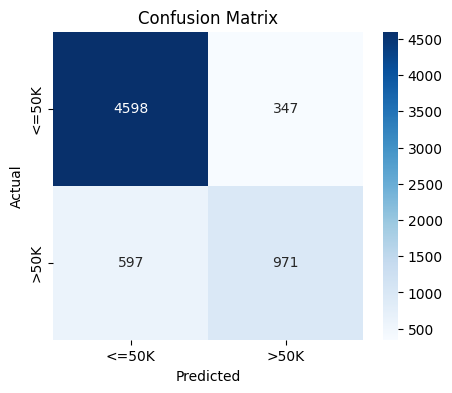
\includegraphics[width=0.5\textwidth]{Q3.png}
    \caption{Confusion Matrix for Logistic Regression Model}
\end{figure}
\newpage
\subsubsection*{Feature Importance: L1 vs L2 Regularization}

The bar chart below compares the top 10 most important features selected by L1 and L2 regularized logistic regression models. L1 tends to zero out coefficients and promote sparsity, while L2 spreads weight across more features.

\begin{figure}[H]
    \centering
    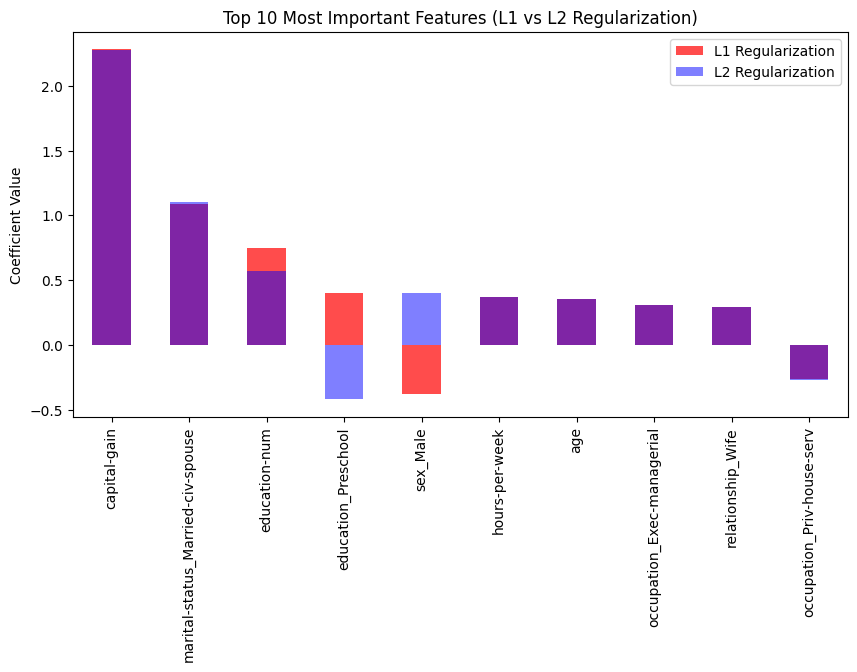
\includegraphics[width=0.8\textwidth]{Q3_1.png}
    \caption{Top 10 Most Important Features (L1 vs L2 Regularization)}
\end{figure}
\newpage
\subsubsection*{ROC Curve and AUC}

The Receiver Operating Characteristic (ROC) curve and the Area Under Curve (AUC) metric give a global view of the model's performance across different thresholds. AUC close to 1 indicates strong classification ability.

\begin{figure}[H]
    \centering
    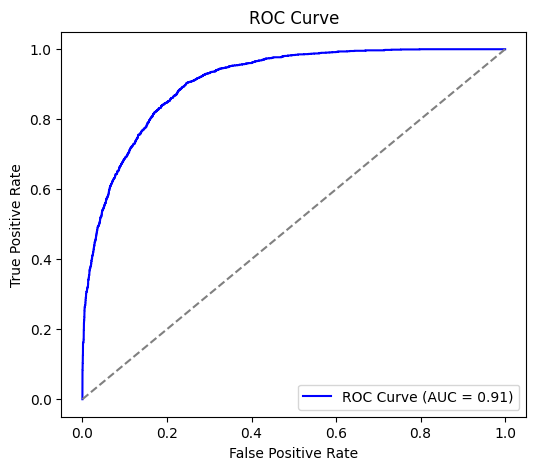
\includegraphics[width=0.6\textwidth]{Q3_2.png}
    \caption{ROC Curve with AUC Score}
\end{figure}
\newpage
\subsubsection*{Precision-Recall vs Threshold}

To determine the optimal classification threshold, the trade-off between precision and recall was analyzed. This plot aids in selecting a threshold that balances false positives and false negatives based on the specific application need.

\begin{figure}[H]
    \centering
    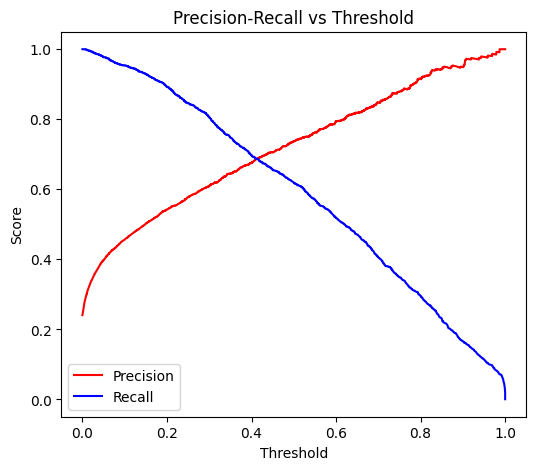
\includegraphics[width=0.6\textwidth]{Q3_3.png}
    \caption{Precision-Recall Curve vs Threshold}
\end{figure}

\newpage
\section{Decision Tree Classifier}

\subsection{Objectives}

The primary objective of this section is to gain a thorough understanding of decision tree learning algorithms. This includes training and evaluating decision trees on different datasets to analyze their performance and interpretability. Additionally, we aim to compare the performance of a single decision tree model against an ensemble of decision trees created using the bagging technique, in order to assess the benefits of model aggregation on classification accuracy and robustness.


\subsection{Dataset}
We used two popular classification datasets:
\begin{itemize}
    \item \textbf{Iris Dataset} – Contains 150 samples from three classes of iris flowers.
    \item \textbf{Wine Dataset} – Contains 178 samples describing chemical properties of wines from three cultivars.
\end{itemize}



\subsection{Approach}

The experimental procedure involved applying decision tree classifiers to two different datasets—\textbf{Iris} and \textbf{Wine}, both available in the \texttt{scikit-learn} library. The following steps were followed in detail:

\begin{enumerate}
    \item \textbf{Data Loading and Splitting:} The Iris and Wine datasets were loaded using \texttt{load\_iris()} and \texttt{load\_wine()} respectively. Each dataset was split into training and testing subsets using an 80/20 ratio with a fixed random state for reproducibility.
    
    \item \textbf{Training Default Decision Trees:} A \texttt{DecisionTreeClassifier} with default hyperparameters was trained on the training set of each dataset.
    
    \item \textbf{Prediction and Evaluation:} Predictions were made on the test sets, and the models were evaluated using accuracy scores, classification reports, and confusion matrices. These metrics allowed for a comprehensive understanding of the performance of each model across different classes.
    
    \item \textbf{Tree Visualization:} The trained decision trees were visualized using the \texttt{plot\_tree()} function. This provided interpretability by showing how the features were used to make splits and how the decision paths were constructed.
    
    \item \textbf{Varying Tree Depths:} To assess the effect of tree complexity on performance, models with different \texttt{max\_depth} values (2, 4, 6, and None) were trained. Accuracy scores for each depth were recorded and plotted to observe trends and potential overfitting or underfitting.
    
    \item \textbf{Ensemble via Bagging:} To improve generalization, a \texttt{BaggingClassifier} with 100 decision tree base estimators was trained on both datasets. This approach creates multiple models trained on random subsets and aggregates their predictions.
    
    \item \textbf{Comparison of Single Tree vs Ensemble:} Finally, the performance of the single default tree was compared against the ensemble bagged model in terms of accuracy on the test set. A bar chart was used to visually compare the results for both datasets.
\end{enumerate}




\subsection{Results}

The performance of the decision tree classifiers was evaluated on the Iris and Wine datasets. The results demonstrated high accuracy, with particularly strong performance on the Iris dataset. Below are the detailed results:

\paragraph{Decision Tree Classifier:}

\begin{itemize}
    \item \textbf{Iris Dataset:}
    \begin{itemize}
        \item Accuracy: 1.00
        \item Precision, Recall, and F1-Score: All perfect (1.00) across all three classes.
    \end{itemize}

    \item \textbf{Wine Dataset:}
    \begin{itemize}
        \item Accuracy: 0.944
        \item Class-wise metrics:
        \begin{itemize}
            \item Class 0: Precision = 0.93, Recall = 0.93, F1-score = 0.93
            \item Class 1: Precision = 0.93, Recall = 1.00, F1-score = 0.97
            \item Class 2: Precision = 1.00, Recall = 0.88, F1-score = 0.93
        \end{itemize}
    \end{itemize}
\end{itemize}

\paragraph{Bagging Ensemble vs. Single Tree Comparison:}

To evaluate whether ensemble methods improved performance, a BaggingClassifier with 100 base estimators was used.

\begin{itemize}
    \item \textbf{Iris Dataset:}
    \begin{itemize}
        \item Single Tree Accuracy: 1.00
        \item Bagging Accuracy: 1.00
        \item Conclusion: No improvement observed, likely due to the dataset being linearly separable and less complex.
    \end{itemize}

    \item \textbf{Wine Dataset:}
    \begin{itemize}
        \item Single Tree Accuracy: 0.944
        \item Bagging Accuracy: 0.972
        \item Conclusion: Ensemble learning improved accuracy by reducing variance and increasing model robustness.
    \end{itemize}
\end{itemize}

Overall, the decision tree classifier showed excellent results, especially when enhanced by ensemble techniques such as bagging, particularly in the more complex Wine dataset.


\subsection{Discussion}

\paragraph{Classification Accuracy and Metrics:}
The performance of decision trees was evaluated on both the Iris and Wine datasets using accuracy, precision, recall, and F1-score. On the Iris dataset, the default decision tree classifier achieved an accuracy of 100\%, indicating perfect classification. This is likely due to the well-separated classes in the Iris dataset. On the Wine dataset, the classifier achieved a slightly lower but still strong accuracy of approximately 94.4\%. The detailed classification report confirmed that all classes were reasonably well predicted, although a minor drop in recall for class 2 was observed.

\paragraph{Tree Visualization and Interpretation:}
The decision trees were visualized using the \texttt{plot\_tree()} function, providing insight into how the models made decisions based on feature values. In both datasets, the tree structure revealed key features that contributed to classification at different levels. For the Iris dataset, features like petal length and width were frequently used near the root, reflecting their strong discriminatory power. Similarly, in the Wine dataset, features like \texttt{flavanoids}, \texttt{color\_intensity}, and \texttt{proline} played critical roles. Tree depth was also observed to influence complexity and interpretability, with deeper trees making more specific splits.

\paragraph{Comparison Between Single Tree and Ensemble Approach:}
To assess whether ensemble learning improves performance, a bagging classifier with 100 decision trees was applied. On the Iris dataset, both the single tree and the ensemble achieved perfect accuracy (100\%), showing that ensemble methods did not provide a benefit due to the simplicity of the classification task. However, for the Wine dataset, the bagging ensemble improved the accuracy from 94.4\% to 97.2\%, demonstrating the ensemble’s ability to reduce variance and improve generalization. The bar plots clearly visualized this gain in accuracy, reinforcing the effectiveness of bagging, especially on more complex datasets.

Overall, decision trees provided strong performance across both datasets, with ensemble methods offering an extra boost on more challenging tasks.


\subsection{Conclusion}
Decision Trees provided interpretable and effective models for classification. The Iris dataset was perfectly separable by a single tree. For more complex datasets like Wine, ensemble methods such as bagging improved generalization and accuracy.

\subsection{Code Implementation}
\begin{lstlisting}[style=python]
    # Import necessary libraries
import numpy as np
import pandas as pd
import matplotlib.pyplot as plt
import seaborn as sns
from sklearn.datasets import load_iris, load_wine
from sklearn.tree import DecisionTreeClassifier, plot_tree
from sklearn.model_selection import train_test_split
from sklearn.metrics import accuracy_score, classification_report, confusion_matrix
from sklearn.ensemble import BaggingClassifier

# Load Iris dataset
iris = load_iris()
X_iris, y_iris = iris.data, iris.target
X_train_iris, X_test_iris, y_train_iris, y_test_iris = train_test_split(X_iris, y_iris, test_size=0.2, random_state=42)

# Load Wine dataset
wine = load_wine()
X_wine, y_wine = wine.data, wine.target
X_train_wine, X_test_wine, y_train_wine, y_test_wine = train_test_split(X_wine, y_wine, test_size=0.2, random_state=42)

# Train Decision Tree Classifier (Default)
dt_iris = DecisionTreeClassifier(random_state=42)
dt_iris.fit(X_train_iris, y_train_iris)

dt_wine = DecisionTreeClassifier(random_state=42)
dt_wine.fit(X_train_wine, y_train_wine)

# Predictions
y_pred_iris = dt_iris.predict(X_test_iris)
y_pred_wine = dt_wine.predict(X_test_wine)

# Evaluate Model Performance
print("=== Decision Tree on Iris Dataset ===")
print("Accuracy:", accuracy_score(y_test_iris, y_pred_iris))
print(classification_report(y_test_iris, y_pred_iris))

print("\n=== Decision Tree on Wine Dataset ===")
print("Accuracy:", accuracy_score(y_test_wine, y_pred_wine))
print(classification_report(y_test_wine, y_pred_wine))

# Confusion Matrices
fig, ax = plt.subplots(1, 2, figsize=(12, 5))
sns.heatmap(confusion_matrix(y_test_iris, y_pred_iris), annot=True, cmap="Blues", fmt="d", ax=ax[0])
ax[0].set_title("Confusion Matrix - Iris")
ax[0].set_xlabel("Predicted")
ax[0].set_ylabel("Actual")

sns.heatmap(confusion_matrix(y_test_wine, y_pred_wine), annot=True, cmap="Reds", fmt="d", ax=ax[1])
ax[1].set_title("Confusion Matrix - Wine")
ax[1].set_xlabel("Predicted")
ax[1].set_ylabel("Actual")

plt.show()

# Visualize Decision Trees
plt.figure(figsize=(12, 6))
plot_tree(dt_iris, feature_names=iris.feature_names, class_names=iris.target_names, filled=True)
plt.title("Decision Tree - Iris Dataset")
plt.show()

plt.figure(figsize=(12, 6))
plot_tree(dt_wine, feature_names=wine.feature_names, class_names=wine.target_names, filled=True)
plt.title("Decision Tree - Wine Dataset")
plt.show()

# Decision Tree with Different Depths
depths = [2, 4, 6, None]  # None means unlimited depth
acc_iris, acc_wine = [], []

for depth in depths:
    dt_iris = DecisionTreeClassifier(max_depth=depth, random_state=42)
    dt_iris.fit(X_train_iris, y_train_iris)
    acc_iris.append(accuracy_score(y_test_iris, dt_iris.predict(X_test_iris)))

    dt_wine = DecisionTreeClassifier(max_depth=depth, random_state=42)
    dt_wine.fit(X_train_wine, y_train_wine)
    acc_wine.append(accuracy_score(y_test_wine, dt_wine.predict(X_test_wine)))

# Plot accuracy vs. tree depth
plt.figure(figsize=(8, 5))
plt.plot(depths, acc_iris, marker="o", label="Iris Dataset", color='blue')
plt.plot(depths, acc_wine, marker="s", label="Wine Dataset", color='red')
plt.xlabel("Tree Depth")
plt.ylabel("Accuracy")
plt.title("Decision Tree Accuracy vs. Depth")
plt.legend()
plt.grid()
plt.show()

# Implement Bagging (Ensemble of Trees)
bagging_iris = BaggingClassifier(DecisionTreeClassifier(), n_estimators=100, random_state=42)
bagging_iris.fit(X_train_iris, y_train_iris)
y_pred_bagging_iris = bagging_iris.predict(X_test_iris)

bagging_wine = BaggingClassifier(DecisionTreeClassifier(), n_estimators=100, random_state=42)
bagging_wine.fit(X_train_wine, y_train_wine)
y_pred_bagging_wine = bagging_wine.predict(X_test_wine)

# Compare Single Decision Tree vs. Bagging
print("\n=== Bagging vs. Single Tree - Iris Dataset ===")
print("Single Tree Accuracy:", accuracy_score(y_test_iris, y_pred_iris))
print("Bagging Accuracy:", accuracy_score(y_test_iris, y_pred_bagging_iris))

print("\n=== Bagging vs. Single Tree - Wine Dataset ===")
print("Single Tree Accuracy:", accuracy_score(y_test_wine, y_pred_wine))
print("Bagging Accuracy:", accuracy_score(y_test_wine, y_pred_bagging_wine))

# Bar Plot to Compare Performance
models = ["Single Tree", "Bagging"]
iris_scores = [accuracy_score(y_test_iris, y_pred_iris), accuracy_score(y_test_iris, y_pred_bagging_iris)]
wine_scores = [accuracy_score(y_test_wine, y_pred_wine), accuracy_score(y_test_wine, y_pred_bagging_wine)]

fig, ax = plt.subplots(1, 2, figsize=(10, 5))
ax[0].bar(models, iris_scores, color=["blue", "green"])
ax[0].set_ylim(0.7, 1.0)
ax[0].set_title("Iris Dataset")
ax[0].set_ylabel("Accuracy")

ax[1].bar(models, wine_scores, color=["red", "purple"])
ax[1].set_ylim(0.7, 1.0)
ax[1].set_title("Wine Dataset")
ax[1].set_ylabel("Accuracy")

plt.show()
\end{lstlisting}

\subsection{Output of Code}
\begin{verbatim}

    === Decision Tree on Iris Dataset ===
Accuracy: 1.0
              precision    recall  f1-score   support

           0       1.00      1.00      1.00        10
           1       1.00      1.00      1.00         9
           2       1.00      1.00      1.00        11

    accuracy                           1.00        30
   macro avg       1.00      1.00      1.00        30
weighted avg       1.00      1.00      1.00        30


=== Decision Tree on Wine Dataset ===
Accuracy: 0.9444444444444444
              precision    recall  f1-score   support

           0       0.93      0.93      0.93        14
           1       0.93      1.00      0.97        14
           2       1.00      0.88      0.93         8

    accuracy                           0.94        36
   macro avg       0.95      0.93      0.94        36
weighted avg       0.95      0.94      0.94        36






=== Bagging vs. Single Tree - Iris Dataset ===
Single Tree Accuracy: 1.0
Bagging Accuracy: 1.0

=== Bagging vs. Single Tree - Wine Dataset ===
Single Tree Accuracy: 0.9444444444444444
Bagging Accuracy: 0.9722222222222222

\end{verbatim}

\subsection{Plots}

\begin{figure}[H]
    \centering
    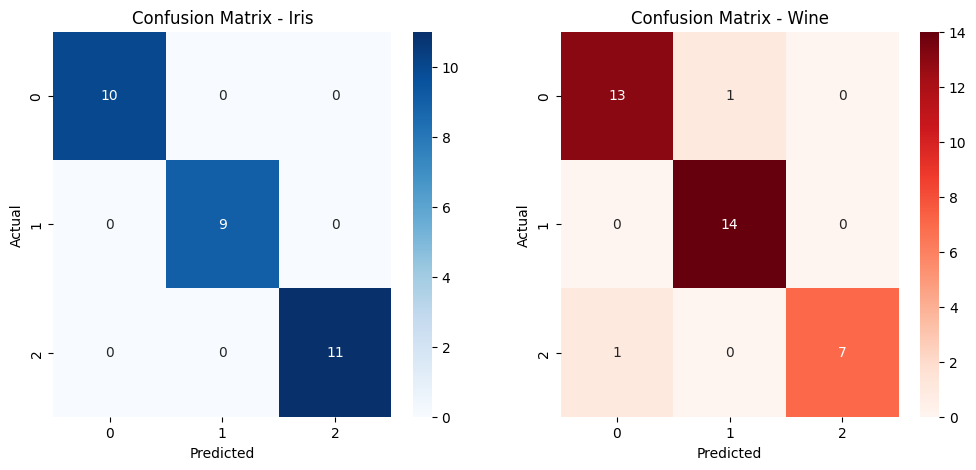
\includegraphics[width=0.9\textwidth]{Q4.png}
    \caption{Confusion Matrices for Iris (left) and Wine (right)}
\end{figure}

\begin{figure}[H]
    \centering
    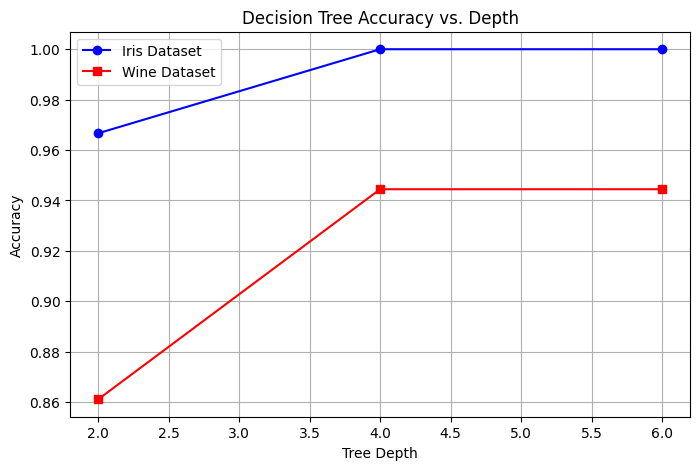
\includegraphics[width=0.9\textwidth]{Q4_4.png}
    \caption{Accuracy vs. Tree Depth for Iris and Wine Datasets}
\end{figure}

\begin{figure}[H]
    \centering
    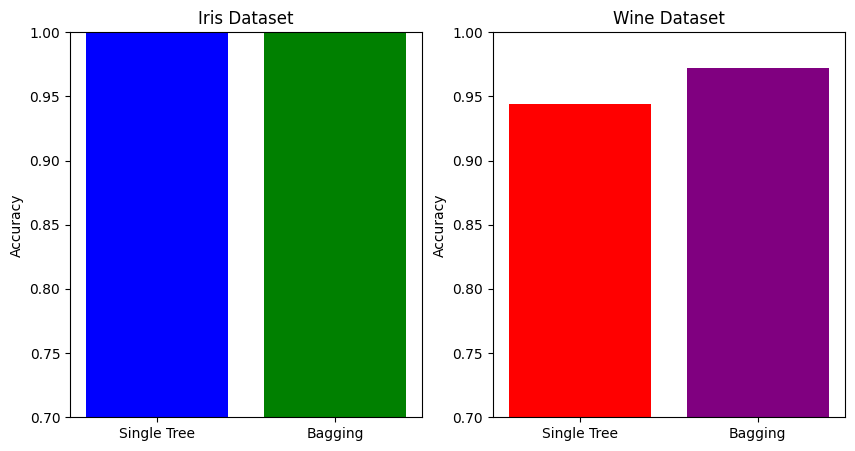
\includegraphics[width=0.8\textwidth]{Q4_5.png}
    \caption{Accuracy Comparison: Single Tree vs. Bagging}
\end{figure}


\begin{figure}[H]
    \centering
    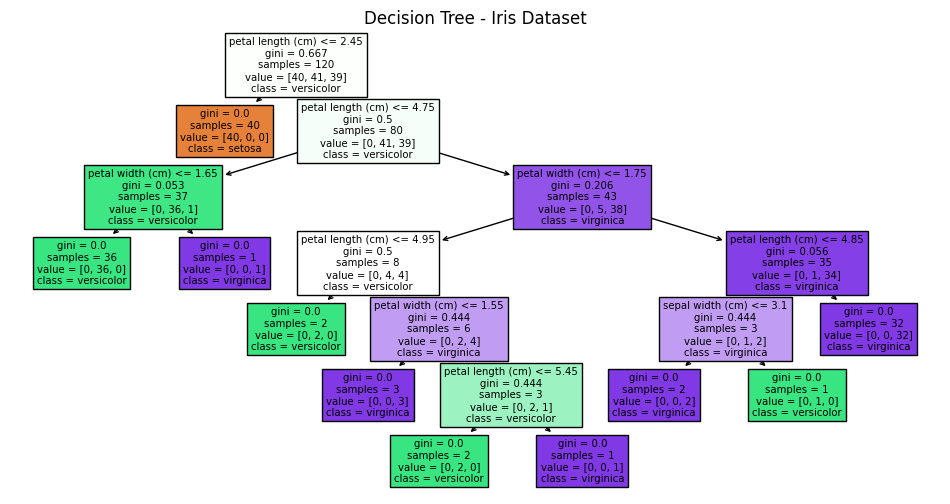
\includegraphics[width=\textwidth]{Q4_2.png}
    \caption{Decision Tree Visualization – Iris Dataset}
\end{figure}

\begin{figure}[H]
    \centering
    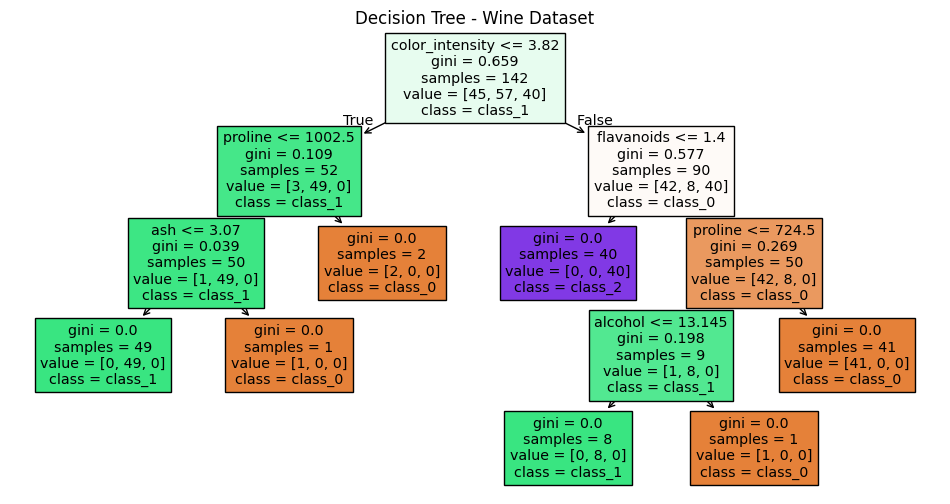
\includegraphics[width=\textwidth]{Q4_3.png}
    \caption{Decision Tree Visualization – Wine Dataset}
\end{figure}



\end{document}
